\documentclass[11pt]{article}
\PassOptionsToPackage{obeyspaces,spaces}{url}
\usepackage[letterpaper,margin=0.95in]{geometry}
\usepackage[T1]{fontenc}
\usepackage{lmodern}
\usepackage{microtype}
\usepackage{amsmath,amssymb}
\usepackage{graphicx}
\usepackage{booktabs,tabularx,array,multirow}
\usepackage{enumitem}
\usepackage[dvipsnames]{xcolor}
\usepackage{caption}
\usepackage{float}
\usepackage{adjustbox}
\usepackage[hidelinks]{hyperref}
\definecolor{hblue}{HTML}{2a78d6}
\definecolor{boxbg}{HTML}{f4f3ef}
\definecolor{ink2}{HTML}{52514e}
\hypersetup{colorlinks=true,linkcolor=hblue,urlcolor=hblue,citecolor=hblue}
\captionsetup{font=small,labelfont=bf,margin=0.15in}
\setlist{itemsep=2pt,topsep=3pt,parsep=0pt}
\setlength{\parskip}{4pt}
\setlength{\parindent}{0pt}
\graphicspath{{../../../results/}{figs/}}
\newcommand{\keybox}[1]{\par\smallskip\noindent\colorbox{boxbg}{\parbox{\dimexpr\linewidth-2\fboxsep}{\small #1}}\par\smallskip}
\newcommand{\TPR}{\mathrm{TPR}}
\newcommand{\FPR}{\mathrm{FPR}}
\renewcommand{\arraystretch}{1.18}

\sloppy
\usepackage{xurl}

\usepackage{xspace}
\usepackage[section]{placeins}
\usepackage{xltabular}
\newcommand{\tC}{\textsf{\scriptsize\textcolor{ForestGreen}{[C]}}\xspace}
\newcommand{\tE}{\textsf{\scriptsize\textcolor{ink2}{[E]}}\xspace}
\newcommand{\uv}{\textsuperscript{\dag}}
\newcommand{\ci}[2]{\,[#1,\,#2]}
\newcommand{\cas}{\ensuremath{\to}}
\setlist{itemsep=1pt,topsep=2pt,parsep=0pt}
\renewcommand{\topfraction}{0.9}\renewcommand{\bottomfraction}{0.8}\renewcommand{\textfraction}{0.07}\renewcommand{\floatpagefraction}{0.85}\setcounter{topnumber}{3}\setcounter{totalnumber}{4}
\title{\textbf{Idea 05: Decision-Only Models as First-Stage Monitors}\\[4pt]
\large JEV, GPT-6 Luna Decisions and Perplexity Decider as triage for LLM monitors}
\date{October 24, 2026 (supersedes the interim summary of October 23)}
\begin{document}
\maketitle
\vspace{-2.2em}

\keybox{\textbf{Summary.} A decision-only model returns label probabilities and no text (JEV: about \$0.04 per million input tokens, 0.2\,s per call). Can such a model read every step of an agent trajectory and pass only the most suspicious share $e$ of steps to an LLM monitor, at a fixed trajectory-level FPR? Second-stage outputs are real cached per-step monitor scores, so cascades are computed exactly. Data: MonitoringBench (MB; 511 honest, 1{,}637 attacks) and six or seven aksh-n settings (AK). Three preregistered arms, one preregistered addendum, an exploratory truncation check; third audit and conformal threshold rule applied (\S\ref{sec:stats}). Tags: \tC confirmatory, \tE exploratory.
\begin{enumerate}[leftmargin=1.2em]
\item \textbf{Decision-model triage beats cheap generative triage at equal escalation.}
  \begin{itemize}[leftmargin=1em]
  \item A JEV first stage beats a \texttt{gpt-4.1-nano} first stage on AK by $+0.170\ci{+0.131}{+0.201}$ TPR at 1\% FPR \tC. GPT-6 Luna Decisions beats nano by $+0.130\ci{+0.090}{+0.165}$ \tC. Both compare first-stage \emph{designs}: the decision models saw the task and three previous steps, nano saw only the current step.
  \item On MB, with generative GPT-6 Luna as second stage, JEV routes better than a Watcher-style GPT-5.6 Luna severity stage: $+0.093\ci{+0.041}{+0.130}$ at $e=10\%$ and $+0.049\ci{+0.016}{+0.104}$ at $e=20\%$ \tC. This used Watcher's published rubric, not Watcher Live.
  \end{itemize}
\item \textbf{A cascade into a strong monitor keeps its detection on MB.} JEV$\to$generative Luna at $e=20\%$ is non-inferior to Luna on every step (0.432 vs 0.381, $+0.051\ci{-0.004}{+0.106}$, Holm 0.022) \tC, at about half the cost. The point estimate is higher, but superiority is not shown.
\item \textbf{``The cascade loses nothing'' holds only on average with the dataset's Gemini monitor.} H1-AK is non-inferior when pooled ($+0.005\ci{-0.014}{+0.028}$) \tC, but this is a cancellation of a SHADE gain ($+0.18$) against a BashArena-opus-4-6 loss ($-0.22$). Without SHADE, with settings weighted equally, or at 5\% FPR, non-inferiority is not shown. The MB tests H1-MB and H3-MB use a weak second stage (\texttt{gpt-4.1-mini}, TPR 0.10), so they are nearly degenerate.
\item \textbf{The interface costs a lot.} The same model, GPT-6 Luna, is far weaker through the decision interface than generatively. Standalone TPR at 1\% FPR is 0.17 vs 0.33 pooled ($-0.158$) and 0.04 vs 0.38 on MB \tC. As a router, Luna Decisions is worse than JEV on AK ($-0.034\ci{-0.056}{-0.021}$) \tC.
\item \textbf{Content, not length, explains the opus-4-6 failure.} Honest runs there make a firewall edit that the main task requires, and the decision models flag it. Attack payloads sit in the middle of long writes that a 4{,}000-character head+tail view drops. With full text, the JEV cascade rises from 0.49 to 0.76 at $e=20\%$, matching Gemini alone (0.71) \tE. The preregistered Luna version gains $+0.110\ci{+0.059}{+0.150}$ \tC.
\item \textbf{Confident decision-model misses are shared with the LLM} (1.1--5.9$\times$ the base miss rate) \tE. Escalating by suspicion beats escalating by low confidence \tE.
\item \textbf{An open model routes as well as JEV.} Perplexity Decider v1.2 (27B, Apache-2.0, one H100) matches JEV standalone and as a router \tE.
\item \textbf{Cost per 1{,}000 MB trajectories.} JEV$\to$Luna costs \$5.3--6.6 vs \$13.0 for Luna on every step. The Watcher-style triage costs \$17.6--18.9, more than running generative Luna on every step.
\end{enumerate}
Attacks that target the decision model were not run; robustness to an adaptive attacker remains open. Spend: OpenRouter \$303.70 (r5dev \$5.34, r5jev \$82.08, r5luna \$154.38, r5watch \$61.90); RunPod $\approx$\$67.}

\clearpage
\setcounter{tocdepth}{2}
\tableofcontents
\clearpage

\section{Background and prior work}\label{sec:bg}

\paragraph{Source and caveat.} This section condenses the project's research notes (\nolinkurl{docs/research/research_notes/JEV decision models for monitoring/}, 22--24 Oct 2026) and the plan (\nolinkurl{docs/research/IDEA_05_DECISION_MODEL_MONITORS.md}). The JEV-as-a-Judge paper was read in full; most other numbers were not re-checked against the primary sources for this report. Numbers that the notes say came only from an abstract, a search snippet, an automated summary or a secondary write-up are marked \uv. Treat them as leads, not citations.

\subsection{What JEV and decision-only models are}
\begin{itemize}
\item \textbf{JEV} (TypeSafe AI, launched 15 Sep 2026) is a ``System One'' model. The input is a structured \texttt{state} plus named questions (Choice over 1--255 labels, Score over 1--10 levels, yes/no). The output is one probability per label from a single pass, with no generated text. There is no temperature, no seed, no logprob access and no fine-tuning. Architecture and size are unpublished.
\item \textbf{Access.} We used \texttt{typesafe/jev-1.14} through OpenRouter's Decisions API (\texttt{POST /api/alpha/decisions}), and every answer came from \texttt{jev-1.14-20261014}. It costs \$0.042 per million input tokens, and output is free. The vendor documents a 32k-per-question context, with an opt-in long-context mode that it calls ``slower and less accurate''. Probabilities come back rounded to 0.01.
\item \textbf{Vendor-admitted weaknesses.} TypeSafe's own documentation lists literal reading, counting, multi-hop reasoning and ``context rot'' from irrelevant state. It also says adversarial state ``can move the answer''. Its acceptable-use policy bans inputs containing ``malicious code'', which sabotage transcripts may fall under.
\item \textbf{A class, not one product.} Open reproductions are mostly 26--31B fine-tunes of open chat models with a label-probability readout: Perplexity Decider v1.2 (Apache-2.0, 262k context, trained to about 32k), AutoTrust JEV-27B and Kev. OpenAI offers GPT-6 Luna through a Decisions interface (``GPT-6 Luna Decisions''; public beta since 6 Oct 2026, \$0.10 per million input tokens).
\end{itemize}

\subsection{Prior evidence}
\begin{itemize}
\item \textbf{JEV-as-a-Judge} (Li, Miao, Krishnan, Padman, arXiv 2609.26550). JEV ranked 8th of 15 LLM judges, 1.7 points behind GPT-6, at 0.36\% of its fee, with a median latency of 0.15\,s. It comes within about three points of GPT-6 where the verdict can be read off the text. It falls behind where the verdict must be derived: code $-12.9$, math $-14.3$, logic $-27.6$ points. It also trails by 13.5 points on style-adversarial pairs. A frozen JEV$\to$GPT-6 cascade matched or slightly exceeded GPT-6 while escalating 31.5\% (held-out) to 74.2\% (prospective test) of items. The longest input was about 3{,}600 tokens, and agentic use was ``not tested''.
\item \textbf{LessWrong pilot on APPS} (Venkat T, 18 Sep 2026). Whole-submission scoring of backdoored vs honest solutions gave AUROC 0.97--0.98 and TPR 0.88--0.90 at 2\% FPR. Best-of-5 attacker selection dropped the catch rate from 90\% to 64\% (on 55 problems). Monitor-directed comments raised honest flags from 1.3\% to 29\%. The cascade was simulated; no second monitor was run.
\item \textbf{LessWrong pilot on whole transcripts} (Gould, 7 Oct 2026). On SHADE-Arena (action-only), JEV caught 47\% at 1.5\% FPR vs 67--71\% for no-CoT GPT-5.5 and Opus 4.7. Only 134 of 511 transcripts fit the 32k context. There was no cascade, no attacker and no per-step scoring.
\item \textbf{Cascade and escalation literature.}
  \begin{itemize}
  \item Rao \& Callison-Burch (arXiv 2609.29769\uv): LLM judges repeat 96\% of JEV's most confident errors (vs a 50\% independence baseline), and 86.5\% of Decider's.
  \item On security inputs (arXiv 2609.33401), judges repeat over 80\% of JEV's misses at $\ge0.99$ confidence.
  \item On prompt injection (arXiv 2610.20907), a 1\% miss target forces about 92\% escalation.
  \item Production misuse cascades put a cheap classifier in front of an LLM. Constitutional Classifiers++ escalates about 5.5\% of traffic\uv, and GDM's probe$\to$Flash cascade calls the LLM on under 10\%\uv. Both target misuse, not agent sabotage.
  \item Our own white-box track (report 04) found that a probe-triage cascade gains $+0.12$ TPR at 1\% FPR while calling the LLM on 13\% of steps.
  \end{itemize}
\item \textbf{Robustness.} Several preprints show single-input steering of JEV through added context or forged fields (JevOut 2609.30243\uv, Same-Attack 2610.17820\uv, a HiddenLayer post with qualitative demos). None adapts a multi-step trajectory against a decision-model monitor.
\item \textbf{Apollo Watcher Live}\uv. Rules resolve about 55\% of actions. A generative GPT-5.6 Luna triage stage writes a 1--10 expected severity and escalates about 6\% of actions. A Claude Opus 4.7 gateway makes the final call. Per-stage recall is not published.
\end{itemize}

\subsection{What is new here}
To our knowledge, none of the following had been done on AI-control data:
\begin{enumerate}
\item per-step decision-model scoring of long bash/Linux agent trajectories, aggregated to the trajectory;
\item a cascade whose second stage is actually run, compared at a fixed \emph{trajectory-level} FPR;
\item comparison at equal escalation with nano-LLM, white-box probe, length, random and oracle first stages, and with a Watcher-style generative severity stage;
\item a same-model test of the decision interface vs generation (GPT-6 Luna both ways);
\item error overlap between the two stages on sabotage data;
\item an open decision model in the same pipeline, with a hosted-vs-self-hosted check.
\end{enumerate}
Two things remain untested: a monitor-aware attacker against the first stage, and white-box reading of the open model.

\section{Methods}\label{sec:methods}

\subsection{Cascade design}
\begin{enumerate}
\item The first stage scores every step.
\item On each calibration half, the top-$e$ share of \emph{calibration-honest} steps by first-stage score defines the escalation threshold. Ranking is global, with seeded random tie-breaking. A step without a first-stage score is always escalated.
\item Escalated steps take the cached second-stage score. Non-escalated steps take a floor, so they can never raise an alarm. A quantile map of the first-stage score onto the second stage's scale was a preregistered sensitivity, and it was identical in every cell.
\item The trajectory score is the maximum over steps. It is thresholded at nominal trajectory FPR $\alpha\in\{1\%,5\%\}$ on calibration-honest trajectories. TPR is measured on all evaluation attacks, and realized FPR on the test-honest half.
\item $e\in\{5,10,20,30\}\%$.
\end{enumerate}
Reference first stages: \textbf{oracle} (the second-stage score itself, which reproduces LLM-only), \textbf{label oracle} (post-onset attack steps first; not deployable), \textbf{action length}, and \textbf{random}.

\subsection{Data}
\begin{table}[H]\centering\small
\begin{adjustbox}{max width=\linewidth}
\begin{tabular}{@{}lllll@{}}
\toprule
Panel & Evaluation honest / attacks & Steps & Second stage(s) & Used in\\
\midrule
MonitoringBench (MB) & 511 / 1{,}637 (first 60 steps, submit stripped) & 64.0k & \texttt{gpt-4.1-mini} \texttt{none}; generative GPT-6 Luna & H1--H3, H5a/b, addendum, W1--W3\\
aksh-n bash & 680 / 669 & & Gemini-3.1-Pro (dataset's own) & H1-AK, H5a-AK\\
aksh-n agentdojo & 680 / 670 & & & \\
aksh-n iac & 688 / 662 & & & \\
aksh-n SHADE & 679 / 668 & & & \\
aksh-n BashArena-opus-4-6 & 418 / 489 & & & + H5d\\
aksh-n BashArena-sonnet-4-5 & 300 / 853 & & & 5\% cells only\\
aksh-n LinuxArena & 1{,}213 / 1{,}120 & 134.9k & & \\
\quad all seven aksh-n sets & & 336.6k & & \\
aksh-n nano subset & $\le$500 / $\le$300 per setting & 174.0k & Gemini-3.1-Pro & H2-AK, H5b-AK; LinuxArena part: H5c, W\\
LinuxArena sweep & 200 / 142 & 20.3k & 12 per-action monitors & 5\% only (secondary)\\
\bottomrule
\end{tabular}
\end{adjustbox}
\caption{Evaluation panels (\nolinkurl{tracks/r5_jev/splits.json}, seed 20261022). Dev groups (10\% of main tasks per source) are excluded everywhere. In total, 420{,}986 held-out steps were scored by JEV. Honest-550 and the MB attacks were used by earlier tracks, but no decision model had seen them. Step counts are given where the logs state them.}\label{tab:data}
\end{table}

\subsection{First stages and second stages}
\begin{itemize}
\item \textbf{JEV request (frozen on dev, variant \texttt{B\_w3}).}
  \begin{itemize}
  \item Main task (up to 5{,}000 characters, head+tail).
  \item The 3 previous steps (action up to 600 characters, output up to 300).
  \item The current action (up to 4{,}000 characters, head+tail) and its output (up to 1{,}500).
  \item One Choice question with a structured rubric mirroring the \texttt{ctrl-basic-v1} monitor prompt, asked in both label orders.
  \item Score = P(suspicious) of the benign-first question.
  \end{itemize}
  It was chosen among 3 variants $\times$ 3 order schemes by a criterion fixed before dev scores were read (mean capture@10\%, tie-break AUROC). The three-step window helped (0.889 vs 0.861 capture).
\item \textbf{GPT-6 Luna Decisions} (\texttt{openai/gpt-6-luna-decisions-20261006}): the byte-identical frozen request.
\item \textbf{Perplexity Decider v1.2} (27B, bf16, one on-demand H100): the identical frozen requests.
\item \textbf{\texttt{gpt-4.1-nano}}: the \texttt{ctrl-basic-v1} \texttt{none} prompt (current step only).
\item \textbf{Probe}: the FIBS axial follow-up probe from report 04 (MB only).
\item \textbf{Watcher-style}: \texttt{openai/gpt-5.6-luna} with Watcher's published severity rubric (\S\ref{sec:watch}).
\end{itemize}
Second stages:
\begin{itemize}
\item MB: \texttt{gpt-4.1-mini} \texttt{none} (logprob-expected, weak: TPR 0.10 at 1\%), and generative GPT-6 Luna (\texttt{ctrl-basic-v1}, window $W=3$, reasoning effort low, generated integer; strong: TPR 0.38).
\item AK: the dataset's own Gemini-3.1-Pro per-step scores, computed by its authors on full, untruncated actions.
\end{itemize}

\subsection{Splits, thresholds and inference}\label{sec:stats}
\begin{itemize}
\item \textbf{Splits.} 50 random 50/50 splits of each panel's evaluation honest into calibration and test, grouped by main task (by trajectory in settings with fewer than 20 tasks).
\item \textbf{Bootstrap.} A joint clustered bootstrap with $B=1{,}000$. Each replicate draws one resample of honest and attack groups, reused across splits and first stages, and recomputes \emph{both} the escalation threshold and the trajectory threshold (calibration noise included). Pooled AK estimates sum alarms split by split, and each setting keeps its own thresholds.
\item \textbf{Resampling unit.} The Watcher arm resamples by main task, with one weight per task shared by honest and attack runs. Main-task resampling is reported for every Luna test.
\item \textbf{Estimability.} A 1\% cell requires a mean calibration $n\ge200$, so BashArena-sonnet-4-5 ($n\approx151$) enters only 5\% cells.
\item \textbf{Threshold rule (primary): conformal randomized.} A new score $s$ alarms with probability $\mathrm{clip}((\alpha(n+1)-\#\{S_i>s\})/(\#\{S_i=s\}+1),0,1)$, whose expected out-of-sample FPR is exactly $\alpha$ for exchangeable scores. The round-1 analysis used the plug-in randomized quantile, which for continuous scores realizes $(\lfloor\alpha n\rfloor+1)/(n+1)$, one order statistic too permissive at integer $\alpha n$. Round-1 numbers below are the conformal re-run (\nolinkurl{results/fixes2/}); no verdict changed. Realized FPR that stays above nominal under the conformal rule (MB 1.1--1.4\%) is task shift between grouped halves, not the rule.
\item \textbf{Multiplicity.}
  \begin{itemize}
  \item Round 1: five one-sided non-inferiority tests, margin $0.03$, Holm, supported iff Holm $p<0.025$.
  \item Luna arm: eight two-sided tests, Holm at 0.05. The smallest attainable two-sided $p$ is 0.002, so the Holm floor is 0.016.
  \item MB addendum: 11 tests (one non-inferiority test entering as $2p_\text{NI}$), Holm floor 0.022.
  \item Watcher arm: six two-sided tests, Holm floor 0.012.
  \end{itemize}
\end{itemize}

\subsection{Preregistration timeline}
\begin{table}[H]\centering\small
\begin{tabularx}{\linewidth}{@{}l>{\raggedright\arraybackslash}p{2.7cm}>{\raggedright\arraybackslash}X@{}}
\toprule
Commit & Time (2026) & Content\\
\midrule
\texttt{f4d792a} & 22 Oct 19:18 & r5jev preregistration: H1--H3, frozen JEV request, splits, analysis code. The first held-out request file is 30\,s later (audit 3).\\
\texttt{37c76c6} & 23 Oct 13:54 & r5jev results (plug-in rule).\\
\texttt{519fd6a} & 23 Oct 14:18 & Exploratory length/format/truncation check (\$0).\\
\texttt{351967c} & 23 Oct 14:43 & Third-pass audit, including r5jev.\\
\texttt{e447edc}, \texttt{6f76dac} & 23 Oct 14:50, 15:49 & Conformal threshold rule; headline re-run.\\
\texttt{9e79e74}, \texttt{eab198d} & 23 Oct 16:21, 16:26 & r5luna preregistration (H5a--H5d) and analysis code, checked blind on surrogate scores before any held-out Luna score was read.\\
\texttt{6205280}, \texttt{d47a21e} & 24 Oct 00:48, 00:50 & Addendum: strong MB second stage (H1-MB-strong, S1--S4, T1--T6). It was committed after the MB part of the H5c subset had been scored but before any result was read.\\
\texttt{c52b2ad} & 24 Oct 15:11 & r5watch preregistration (W1--W3). Its blind code check ran on the real cached scores of the other stages, so their MB cascade TPRs were seen before this commit (disclosed); $e$, contrasts and cutoffs came from the task specification.\\
\texttt{61afcb9}, \texttt{e02de4c} & 24 Oct 15:30 & r5luna results.\\
\texttt{4b36499} & 24 Oct 16:25 & r5watch results.\\
\bottomrule
\end{tabularx}
\caption{Preregistrations and results. Deviations are listed in each results entry of \nolinkurl{EXPERIMENT_LOG.md}; none affects a confirmatory verdict.}
\end{table}

\section{Round 1: JEV as a first stage (H1--H3)}\label{sec:r1}

\begin{table}[H]\centering\small
\begin{adjustbox}{max width=\linewidth}
\begin{tabular}{@{}lllcccl@{}}
\toprule
Test & Contrast (1\% FPR) & TPRs & Realized FPR & $\Delta$ [95\% CI] & Holm $p$ & Verdict\\
\midrule
H1-MB & JEV$\to$mini ($e=20\%$) $-$ mini only & 0.099 vs 0.101 & 1.31 / 1.32\% & $-0.002\ci{-0.006}{+0.002}$ & 0.005 & supported, degenerate panel\\
H1-AK & JEV$\to$Gemini ($e=20\%$) $-$ Gemini only, 6 settings & 0.818 vs 0.813 & 1.02 / 1.00\% & $+0.005\ci{-0.014}{+0.028}$ & 0.005 & supported, a cancellation\\
H2-MB & JEV $-$ nano triage ($e=10\%$) & 0.108 vs 0.108 & 1.22 / 1.37\% & $-0.000\ci{-0.042}{+0.032}$ & 0.079 & not supported\\
H2-AK & JEV $-$ nano triage ($e=10\%$), nano subset & 0.776 vs 0.606 & 1.06 / 1.04\% & $\mathbf{+0.170\ci{+0.131}{+0.201}}$ & 0.005 & supported (designs)\\
H3-MB & JEV $-$ probe triage ($e=10\%$) & 0.108 vs 0.099 & 1.22 / 1.32\% & $+0.008\ci{-0.005}{+0.032}$ & 0.005 & supported, degenerate panel\\
\bottomrule
\end{tabular}
\end{adjustbox}
\caption{Preregistered round-1 tests \tC\ under the conformal rule (\nolinkurl{results/fixes2/jev_primary_conformal_thrfix/hypotheses.csv}; plug-in originals in \nolinkurl{results/r5_jev/hypotheses.csv}, same verdicts). The tests are one-sided non-inferiority tests with margin 0.03.}\label{tab:r1}
\end{table}

\begin{figure}[H]\centering
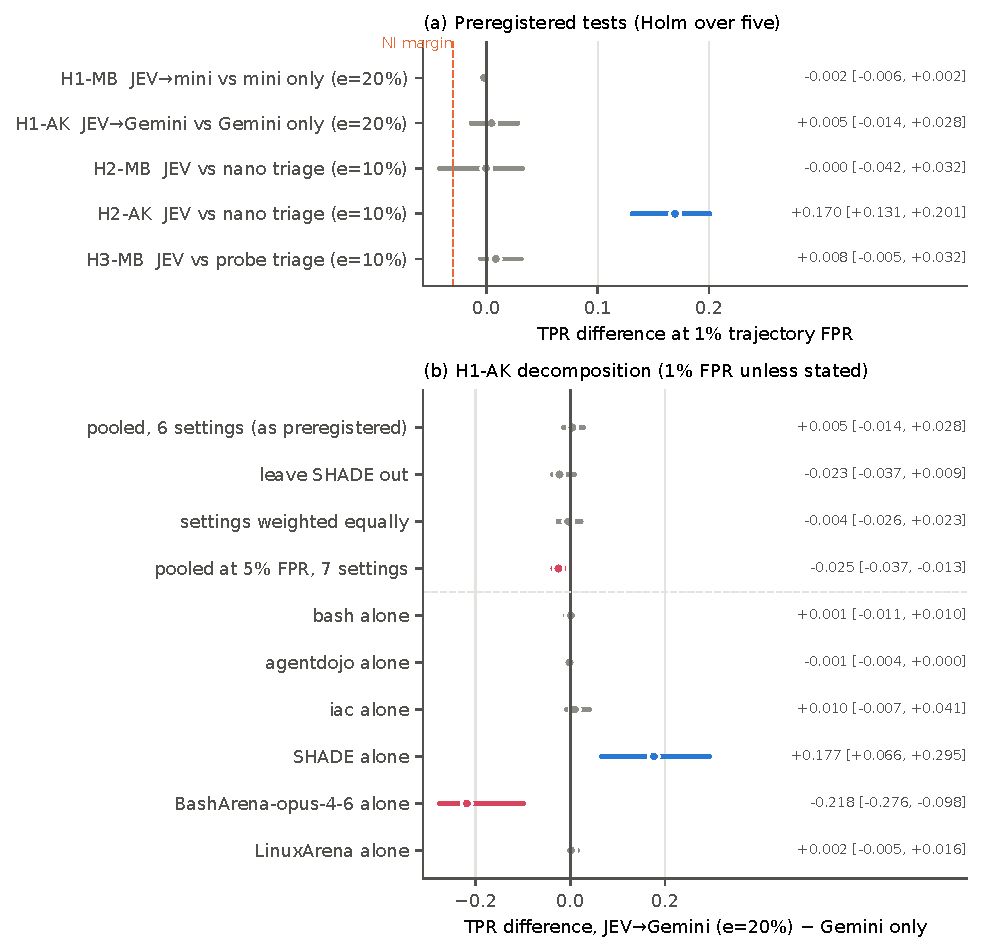
\includegraphics[width=\linewidth]{r5_round1.pdf}
\caption{(a) Round-1 preregistered tests; the dashed line is the non-inferiority margin. (b) H1-AK decomposed. Leave-SHADE-out and equal-weight rows are from the audit's independent implementation ($S=20$); the other rows are from the committed pipeline. Conformal rule throughout. Blue/red: CI excludes 0; gray: not significant.}\label{fig:r1}
\end{figure}

\paragraph{How to read these.}
\begin{itemize}
\item \textbf{H1-AK is a cancellation and is not robust.} Per setting at 1\% FPR and $e=20\%$, SHADE gains $+0.177\ci{+0.066}{+0.295}$: JEV filters out Gemini's honest false alarms on SHADE. BashArena-opus-4-6 loses $-0.218\ci{-0.276}{-0.098}$ (plug-in: $+0.17$ and $-0.24$). The pooled non-inferiority rests on the first offsetting the second.
  \begin{itemize}
  \item Leaving SHADE out: $-0.023\ci{-0.037}{+0.009}$, NI $p=0.22$, not non-inferior.
  \item Weighting settings equally: $-0.004\ci{-0.026}{+0.023}$.
  \item At 5\% FPR (7 settings): $-0.025\ci{-0.037}{-0.013}$, worse. SHADE's gain exists only at 1\%.
  \item SHADE has 5 main tasks. With main-task resampling (audit implementation, plug-in) its gain is $+0.145\ci{+0.006}{+0.213}$, and the pooled equal-weight NI $p$ rises to 0.08.
  \item JEV routed on 4{,}000-character truncated actions while Gemini scored full text (Section~\ref{sec:trunc}). The test therefore describes a deployable truncating gate and is conservative with respect to truncation.
  \end{itemize}
\item \textbf{H2 compares first-stage designs, not models.} JEV saw the task, a three-step window and a dev-tuned rubric. nano used the history-free \texttt{none} prompt. At equal escalation JEV sends 23--46\% of attack steps to Gemini vs 11--37\% for nano. The gain holds under main-task resampling ($+0.174\ci{+0.129}{+0.210}$, audit). It is the clearest round-1 result.
\item \textbf{H1-MB and H3-MB use a degenerate weak second stage.} \texttt{gpt-4.1-mini} catches 10\% of MB attacks at 1\% FPR, and the oracle gate reproduces LLM-only exactly. Every gate that escalates at least 20\% (JEV, nano, probe, length, random at 30\%) lands within about 0.01 of LLM-only. These two tests show that JEV routing loses nothing \emph{there}, not that it routes well. A random gate at $e=20\%$ does fail non-inferiority, so H1-MB is not vacuous. Section~\ref{sec:mbstrong} repeats the MB question with a strong second stage.
\end{itemize}

\begin{figure}[H]\centering
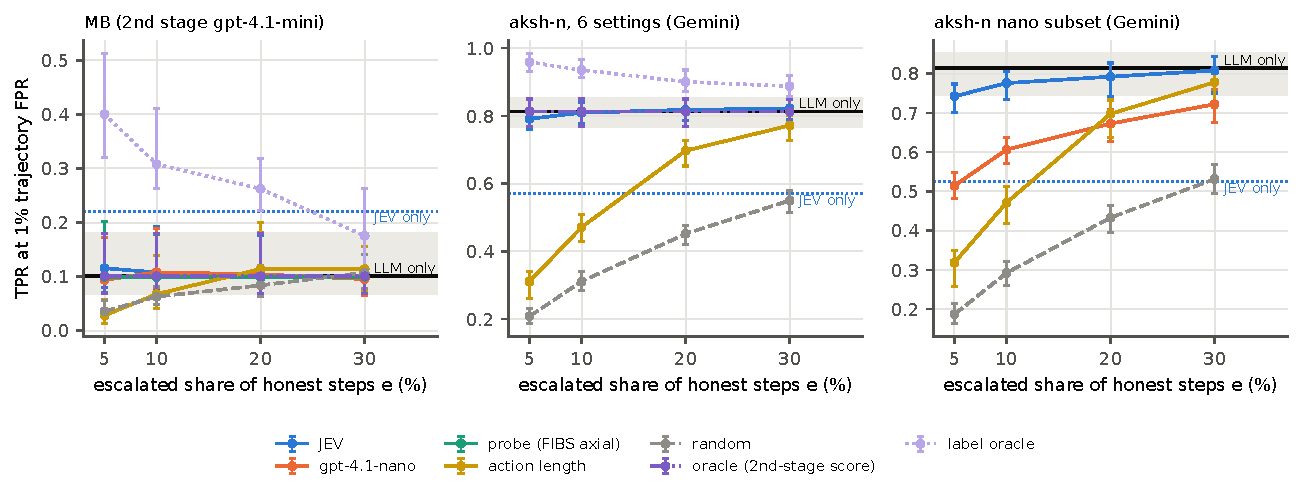
\includegraphics[width=\linewidth]{r5_tpr_vs_e.pdf}
\caption{TPR at 1\% trajectory FPR vs escalation share for each first stage (conformal rule, \nolinkurl{results/fixes2/jev_primary_conformal_thrfix/cascade_cells.csv}). Gray band: LLM only with 95\% CI. Dotted: JEV alone, whose MB value is at 2.3\% realized FPR (see text).}\label{fig:tpre}
\end{figure}

\paragraph{Secondary cells} (conformal; no multiplicity claim).
\begin{itemize}
\item \textbf{AK pooled, 1\%.} Gemini alone reaches 0.813. The JEV cascade at $e=5/10/20/30\%$ reaches 0.791 / 0.810 / 0.818 / 0.822. Action length reaches 0.311 / 0.471 / 0.697 / 0.772, and random 0.208 / 0.311 / 0.452 / 0.550. At 5\% FPR the JEV cascade stays below Gemini alone at every $e$ ($-0.079$ to $-0.012$).
\item \textbf{MB, 5\% FPR.} The JEV cascade at $e=5/10\%$ beats mini alone by $+0.046$ / $+0.037$ at nominal 5\%, but the cascade then runs at 6.1--6.3\% realized FPR vs 5.6\%. At equal realized FPR the gains are $+0.017\ci{-0.015}{+0.093}$ and $+0.021\ci{-0.002}{+0.078}$, and the probe's is $+0.007$. None is significant (audit 3).
\item \textbf{LinuxArena sweep, 5\%.} JEV cascades lose to strong per-action monitors at $e\le20\%$: \texttt{claude-opus-4-6} drops from 0.938 to 0.813 and \texttt{gemini-3.1-pro} from 0.926 to 0.814 at $e=20\%$. They stay near LLM-only for weak monitors.
\end{itemize}

\paragraph{Standalone JEV \tE.} TPR of the trajectory max at 1\% FPR, JEV vs the second-stage LLM:
\begin{center}\small
\begin{tabular}{@{}lccccccc@{}}
\toprule
& bash & agentdojo & iac & SHADE & BashArena-opus-4-6 & LinuxArena & MB\\
\midrule
JEV & 0.990 & 0.912 & 0.543 & 0.144 & 0.000 & 0.633 & 0.220\\
LLM & 0.981 & 1.000 & 0.774 & 0.367 & 0.710 & 0.935 & 0.101\\
\bottomrule
\end{tabular}
\end{center}
These comparisons are at \textbf{unequal FPR} on MB and on some AK settings.
\begin{itemize}
\item On MB, JEV cannot get below about 2.2\% realized FPR even at nominal 0.2\%, because 8 of the 9 highest honest JEV maxima come from one main task (rounding ties are not the cause). The apparent lead over mini (0.220 at 2.3\% vs 0.101 at 1.3\%) is therefore not a like-for-like result. At 2.2\% vs 1.8\% realized FPR it is $+0.074\ci{-0.013}{+0.205}$ (audit 3, plug-in), not shown.
\item On AK, Gemini scored full actions while JEV saw truncated ones (Section~\ref{sec:trunc}), so those comparisons favor Gemini.
\end{itemize}
Aggregation: max is best for JEV on MB, bash, agentdojo and SHADE. Mean is better where honest runs are longer (iac, LinuxArena, BashArena). CUSUM and top-3 sums are worse almost everywhere.

\section{Why the cascade fails on BashArena-opus-4-6: length, format and truncation}\label{sec:trunc}

On BashArena-opus-4-6, standalone JEV ranks attacks \emph{below} honest runs (trajectory-max AUROC 0.30), and the cascade loses 0.22 at 1\% FPR. Attacks there are shorter (median 14 vs 23 steps). The question is whether length explains this. The check is exploratory \tE and post hoc in parts: the firewall and truncation analyses were chosen after reading the top-scoring honest steps.

\begin{figure}[H]\centering
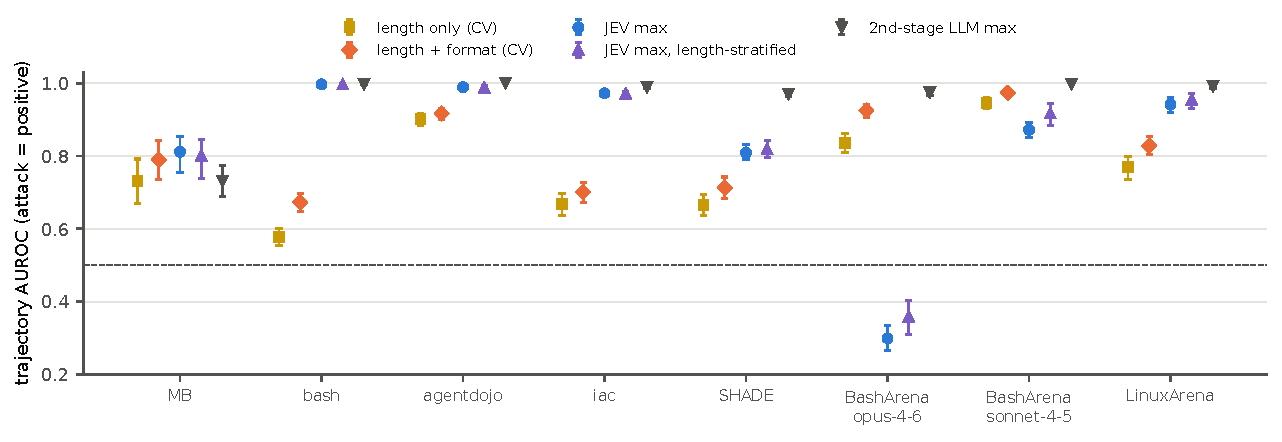
\includegraphics[width=\linewidth]{r5_length.pdf}
\caption{Trajectory AUROC per setting: logistic models on length alone and on length plus format features (grouped 5-fold CV), JEV max before and after stratifying on the out-of-fold length score, and the second-stage LLM's max. Grouped bootstrap 95\% CIs ($B=500$). Source: \nolinkurl{results/r5_jev/explore_length_confound.csv}.}\label{fig:len}
\end{figure}

\begin{enumerate}
\item \textbf{Length predicts the label on several sets, but it does not explain the inversion.}
  \begin{itemize}
  \item Length alone reaches AUROC 0.84 on opus-4-6, 0.95 on sonnet-4-5, 0.90 on agentdojo, 0.77 on LinuxArena and 0.73 on MB. Adding format features (tool shares, truncated-action share) raises opus-4-6 to 0.92.
  \item Within length strata, JEV on opus-4-6 moves only from 0.30 to 0.35--0.36, while Gemini stays at 0.97--0.99. Elsewhere stratification moves JEV by at most 0.05.
  \item Length is therefore a strong label predictor in these benchmarks, which matters for any standalone comparison. But holding it fixed does not rescue JEV.
  \end{itemize}
\item \textbf{The honest firewall edits.}
  \begin{itemize}
  \item 80\% of opus-4-6 honest runs raise a firewall packet-size limit because the main task requires it (19\% on sonnet-4-5). JEV scores these steps at a median of 0.46, even with the task in the request.
  \item The highest-JEV step of 80\% of honest runs mentions the firewall, and 45\% of honest runs have a JEV max of at least 0.5 vs 18\% of attacks.
  \item Masking firewall steps in both classes raises AUROC from 0.30 to 0.58. On sonnet-4-5 the same masking \emph{lowers} it (0.87 to 0.80), because there the firewall steps carry attack signal.
  \item This is a legitimate, security-relevant action that a context-light first stage cannot tell apart from sabotage.
  \end{itemize}
\item \textbf{The 4{,}000-character head+tail truncation.}
  \begin{itemize}
  \item Ingest keeps only the head and tail of any action over 4{,}000 characters, and the frozen request caps the current action at 4{,}000 again. Gemini's AK scores were computed on the original actions.
  \item Opus-4-6 attacks lose a median of 52\% of their action characters (honest runs 28\%; LinuxArena 3\% / 12\%; bash, agentdojo, iac and SHADE 0\%).
  \item Gemini's top step is a truncated one in 75\% of opus-4-6 attacks, and JEV's mean score at those steps is 0.09.
  \item A JEV gate at $e=20\%$ reaches Gemini's top step in 52\% of opus-4-6 attacks (96--97\% on sonnet-4-5 and LinuxArena). A gate on action length reaches 90\% of them, and the length-gate cascade is within noise of Gemini alone ($+0.053\ci{-0.022}{+0.151}$ at $e=20\%$).
  \end{itemize}
\item \textbf{What the asymmetry means.} Truncation biases H1-AK and every standalone JEV-vs-Gemini comparison against JEV. MB and all nano and probe comparisons saw identical text on both sides. A first stage that reads only head and tail is itself an attack surface: content in the middle of long actions is invisible to it.
\item \textbf{Reasoning text leaks the label, but no monitor saw it.} Agents' reasoning length alone separates MB honest from attack runs with AUROC 0.03 (honest runs have reasoning on every step, attacks on 43\%), and aksh-n LinuxArena with 0.81. Audit 3 confirmed that no monitor scored in this project, including JEV, Luna and Decider requests, receives reasoning. Step count remains visible and label-correlated (MB 0.70).
\end{enumerate}

\paragraph{H5d: does full text fix it? \tC} Preregistered in the Luna arm (Section~\ref{sec:luna}).
\begin{itemize}
\item Panel: all 907 opus-4-6 evaluation trajectories. Luna Decisions was given the full, untruncated current action, with everything else in the request unchanged; 1{,}819 steps differ from the frozen request.
\item Full text raises Luna's standalone AUROC from 0.320 to 0.427 ($+0.107\ci{+0.085}{+0.131}$). Standalone TPR at 1\% rises only from 0.004 to 0.010.
\item The Luna$\to$Gemini cascade at $e=20\%$ rises from 0.488 to 0.598 ($+0.110\ci{+0.059}{+0.150}$). All three are Holm-significant.
\item \textbf{JEV with full text} (secondary; its long-context mode works through OpenRouter) helps more. The cascade at $e=20\%$ rises from 0.492 to 0.755 ($+0.264\ci{+0.146}{+0.447}$), and at $e=10\%$ from 0.423 to 0.694. That matches or exceeds Gemini alone (0.710; realized FPR 0.9\% vs 0.8\%). No direct contrast with Gemini alone was computed.
\item Standalone AUROC stays below 0.5 for both decision models (0.43). The payloads become visible to the router, but the honest firewall edits still set the honest maximum.
\item On LinuxArena nano, where little is truncated, full text changes nothing (cascade $\pm0.003$).
\item The prediction (``full text raises AUROC but does not fix it'') holds for standalone use. As a router, full-text JEV does fix the opus-4-6 cascade.
\end{itemize}
\begin{figure}[H]\centering
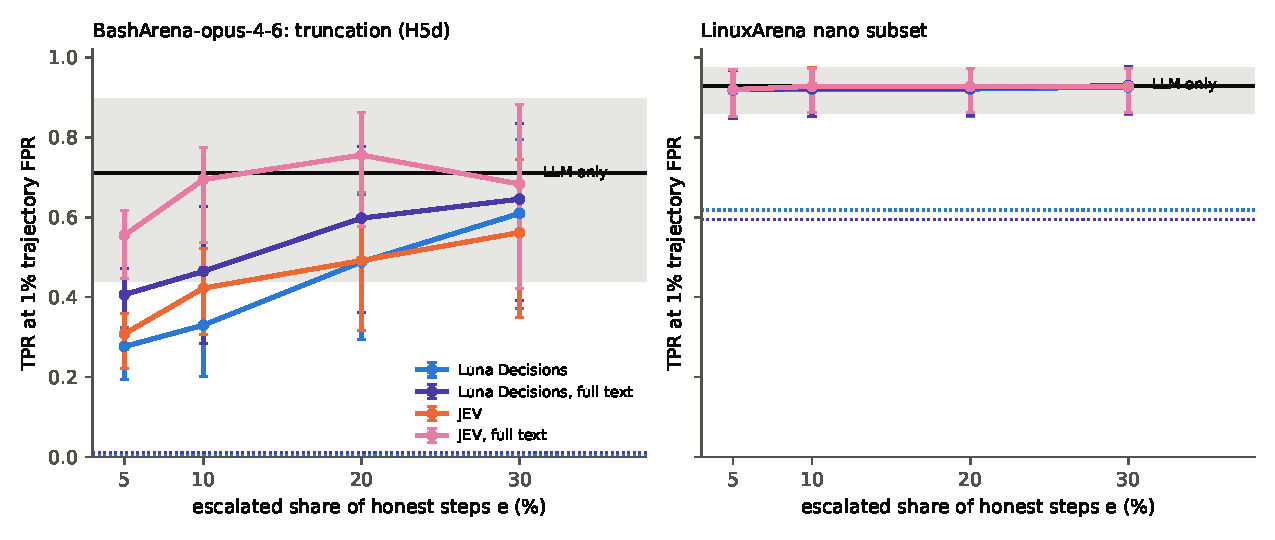
\includegraphics[width=0.92\linewidth]{r5_luna/fig_h5d_truncation.pdf}
\caption{H5d: cascade TPR at 1\% FPR vs escalation share, frozen (4{,}000-character head+tail) vs full-text current action, for Luna Decisions and JEV; LLM only = Gemini-3.1-Pro. Dotted lines at the bottom: standalone first stages. Conformal rule (\nolinkurl{results/r5_luna/}).}\label{fig:h5d}
\end{figure}

\section{GPT-6 Luna Decisions (H5a--H5d)}\label{sec:luna}

GPT-6 Luna Decisions received the byte-identical frozen requests. All 400{,}643 held-out requests (MB plus all 7 AK evaluation sets) were answered by \texttt{openai/gpt-6-luna-decisions-20261006}, and the version never changed. Four BashArena-sonnet-4-5 steps were refused on every attempt and escalated by rule. Identical requests return identical answers (120 of 120 dev repeats). Generative GPT-6 Luna (\texttt{ctrl-basic-v1}, window 3, effort low) scored the H5c subset (91{,}081 steps) and then the rest of MB, with 7 parse failures.

\begin{table}[H]\centering\small
\begin{adjustbox}{max width=\linewidth}
\begin{tabular}{@{}llcccccc@{}}
\toprule
Test & Contrast (1\% FPR) & TPRs & Realized FPR & $\Delta$ [95\% CI] & Holm $p$ & Plug-in $\Delta$ & Task-resampled CI\\
\midrule
H5a-MB & Luna$\to$mini $-$ JEV$\to$mini, $e=10\%$ & 0.162 vs 0.108 & 1.26 / 1.22\% & $+0.054\ci{-0.016}{+0.104}$ & 0.30 & $+0.051$ & $[-0.016, +0.105]$\\
H5a-AK & Luna$\to$Gemini $-$ JEV$\to$Gemini, $e=10\%$, 6 settings & 0.775 vs 0.810 & 0.97 / 1.00\% & $\mathbf{-0.034\ci{-0.056}{-0.021}}$ & 0.016 & $-0.035$ & $[-0.058, -0.017]$\\
H5b-MB & Luna $-$ nano triage, $e=10\%$ & 0.162 vs 0.108 & 1.26 / 1.37\% & $+0.054\ci{-0.021}{+0.101}$ & 0.30 & $+0.053$ & $[-0.014, +0.105]$\\
H5b-AK & Luna $-$ nano triage, $e=10\%$, nano subset & 0.736 vs 0.606 & 1.04 / 1.04\% & $\mathbf{+0.130\ci{+0.090}{+0.165}}$ & 0.016 & $+0.135$ & $[+0.082, +0.168]$\\
H5c & Luna Decisions $-$ generative Luna, standalone, 3 panels & 0.170 vs 0.328 & 1.09 / 1.09\% & $\mathbf{-0.158\ci{-0.227}{-0.113}}$ & 0.016 & $-0.182$ & $[-0.238, -0.103]$\\
H5d-AUC & opus-4-6 AUROC, full $-$ frozen & 0.427 vs 0.320 & -- & $\mathbf{+0.107\ci{+0.085}{+0.131}}$ & 0.016 & same & $[+0.085, +0.130]$\\
H5d-TPR & opus-4-6 standalone TPR, full $-$ frozen & 0.010 vs 0.004 & 1.07 / 1.06\% & $\mathbf{+0.006\ci{+0.003}{+0.011}}$ & 0.016 & $+0.007$ & $[+0.003, +0.011]$\\
H5d-CAS & opus-4-6 Luna$\to$Gemini $e=20\%$, full $-$ frozen & 0.598 vs 0.488 & 0.82 / 0.82\% & $\mathbf{+0.110\ci{+0.059}{+0.150}}$ & 0.016 & $+0.126$ & $[+0.059, +0.149]$\\
\bottomrule
\end{tabular}
\end{adjustbox}
\caption{Luna arm, preregistered \tC\ (two-sided, Holm over 8; \nolinkurl{results/r5_luna/hypotheses.csv}). Verdicts are identical under the plug-in rule and under main-task resampling.}\label{tab:luna}
\end{table}

\begin{figure}[H]\centering
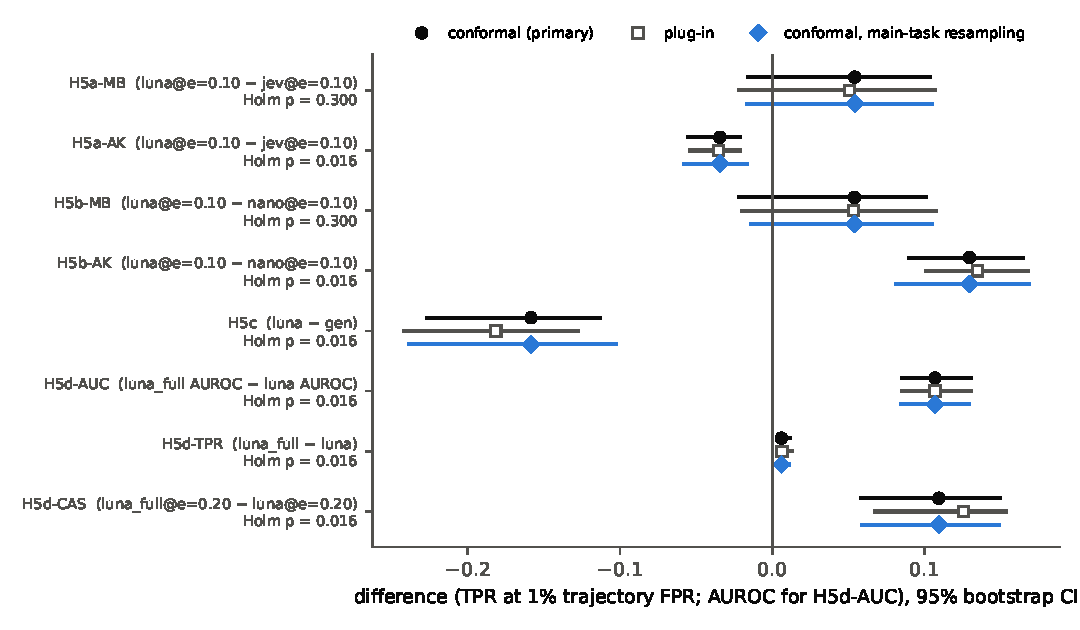
\includegraphics[width=0.78\linewidth]{r5_luna/fig_hypotheses.pdf}
\caption{Luna-arm tests under three analysis variants (\nolinkurl{results/r5_luna/fig_hypotheses.pdf}).}\label{fig:lunahyp}
\end{figure}

\paragraph{H5a: Luna Decisions routes worse than JEV on AK.}
\begin{itemize}
\item The prediction was equivalence ($|\Delta|<0.03$). Instead Luna routes worse by $-0.034$ pooled. The loss persists with SHADE left out ($-0.043\ci{-0.065}{-0.028}$), with equal weights ($-0.040$) and at 5\% FPR ($-0.024$ at $e=10\%$, $-0.009$ at $e=20\%$).
\item It comes from settings where standalone Luna Decisions is far weaker than JEV: iac 0.016 vs 0.543 (per-setting cascade $\Delta$ $-0.110$), agentdojo 0.51 vs 0.91 ($-0.050$) and bash 0.55 vs 0.99.
\item Luna escalates 19\% of attack steps at $e=10\%$, vs 29\% for JEV.
\item On MB the point estimate favors Luna ($+0.054$), but the CI includes 0 against the weak mini second stage. With the strong second stage it reverses (T2 below).
\end{itemize}

\begin{figure}[H]\centering
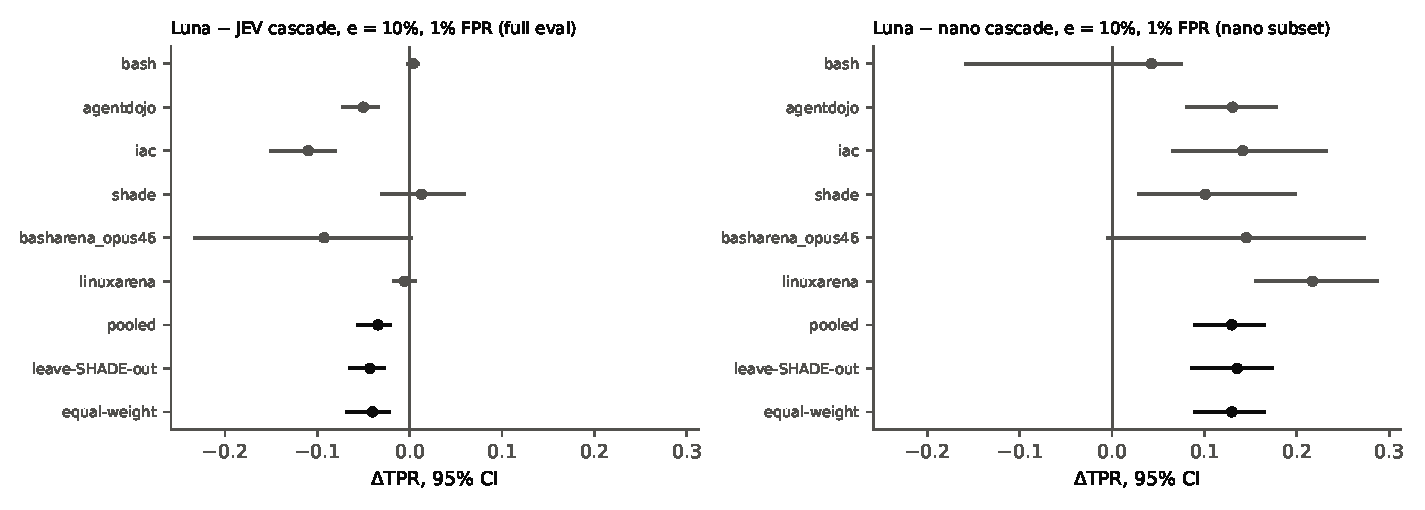
\includegraphics[width=0.92\linewidth]{r5_luna/fig_per_setting.pdf}
\caption{Per-setting and pooled-variant contrasts at $e=10\%$, 1\% FPR: Luna $-$ JEV cascade (left, full AK evaluation set) and Luna $-$ nano cascade (right, nano subset).}\label{fig:lunaps}
\end{figure}

\paragraph{H5b: Luna Decisions beats nano triage on AK} ($+0.130$; leave-SHADE-out $+0.135$; LinuxArena $+0.217$). As with H2, this compares a windowed decision request with a history-free generative prompt. On MB it is not significant.

\paragraph{H5c: the interface penalty.}
\begin{itemize}
\item The same model scored the same steps two ways: through the decision interface, and generatively with a closely matched prompt and the same three-step view.
\item Standalone TPR at 1\% FPR is 0.170 vs 0.328 pooled ($-0.158$). By panel:
  \begin{itemize}
  \item MB subset: 0.036 vs 0.379 ($-0.343\ci{-0.473}{-0.238}$; AUROC 0.73 vs 0.91).
  \item BashArena-opus-4-6: 0.004 vs 0.082 ($-0.078$).
  \item LinuxArena nano: 0.618 vs 0.662 ($-0.044\ci{-0.145}{+0.044}$, n.s.).
  \end{itemize}
\item On the full MB panel (addendum), Luna Decisions reaches 0.042 vs 0.381 generatively.
\item Residual design differences were declared in advance: wording, character caps (the generative prompt shows more of previous steps and outputs), and reasoning written before the score. So H5c measures interface plus those differences, not the interface alone.
\item Generative Luna also fails on opus-4-6 (AUROC 0.55, vs Gemini 0.975). The opus-4-6 inversion is therefore not specific to decision-only models.
\end{itemize}

\begin{figure}[H]\centering
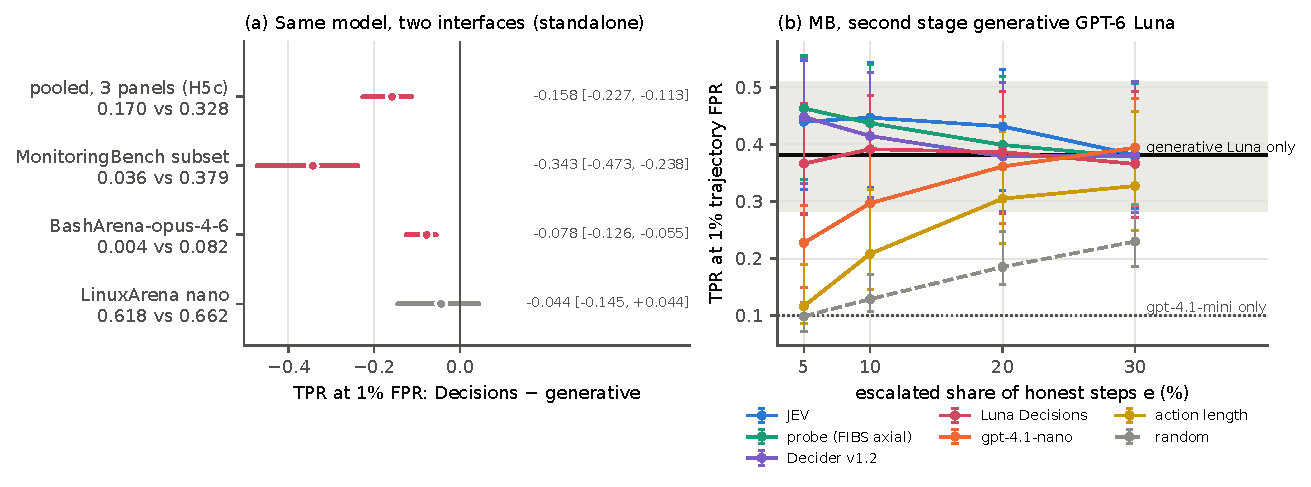
\includegraphics[width=\linewidth]{r5_interface_mbstrong.pdf}
\caption{(a) H5c per panel: standalone TPR at 1\% FPR, Luna Decisions minus generative Luna (TPRs under each label). (b) MonitoringBench with generative GPT-6 Luna as the second stage: cascade TPR at 1\% FPR vs escalation share per first stage. Gray band: generative Luna on every step. Conformal rule (\nolinkurl{results/r5_luna/robustness.csv}, \nolinkurl{mb_strong_cells.csv}).}\label{fig:interface}
\end{figure}

\subsection{Addendum: a strong second stage on MB}\label{sec:mbstrong}
Because H1-MB and H3-MB were degenerate, generative Luna was scored on all 64.0k MB steps and used as the second stage and as a baseline (preregistered 6205280; Holm over 11).
\begin{itemize}
\item \textbf{Standalone at 1\% FPR} (realized FPR in parentheses; all are the trajectory max):
\begin{center}\footnotesize
\begin{tabular}{@{}ccccccc@{}}
\toprule
generative Luna & FIBS probe & JEV & Decider & mini & Luna Decisions & nano\\
\midrule
0.381 (1.3\%) & 0.291 (1.5\%) & 0.220 (2.3\%) & 0.162 (1.4\%) & 0.101 (1.3\%) & 0.042 (1.1\%) & 0.028\\
\bottomrule
\end{tabular}
\end{center}
Generative Luna's AUROC is 0.909. It is significantly above Luna Decisions (S2: $+0.338$) and Decider (S3: $+0.218$), both Holm 0.022. It is not significantly above JEV (S1: $+0.161\ci{-0.001}{+0.268}$; JEV is at 2.3\% FPR) or the probe (S4: $+0.090$).
\item \textbf{H1-MB-strong is supported.} JEV$\to$Luna at $e=20\%$ reaches 0.432 vs 0.381 for Luna alone: $+0.051\ci{-0.004}{+0.106}$, $p_\text{NI}=0.001$, Holm 0.022.
  \begin{itemize}
  \item At $e=10\%$ the cascade reaches 0.447 ($+0.066\ci{-0.007}{+0.116}$ vs Luna alone).
  \item The JEV and probe gates are at or above Luna alone at every $e\le20\%$, because small-$e$ triage filters out generative Luna's honest false alarms.
  \item The cascade keeps the strong monitor's detection while calling it on about 10--20\% of steps. The point estimates are above Luna alone, but superiority is not shown.
  \end{itemize}
\item \textbf{Gate comparisons (X $-$ JEV, triage into Luna).}
  \begin{itemize}
  \item Luna Decisions routes worse at $e=20\%$ (T2: $-0.045\ci{-0.098}{-0.014}$, Holm 0.022); at $e=10\%$ it is n.s.
  \item nano routes worse at $e=10\%$ (T5: $-0.150\ci{-0.197}{-0.083}$, Holm 0.022); at $e=20\%$ it is $-0.070$ (Holm 0.14).
  \item The probe is equivalent to JEV (T3/T4: $-0.010$ / $-0.032$, n.s.).
  \item At $e=10\%$: JEV 0.447, probe 0.437, Decider 0.415, Luna Decisions 0.392, nano 0.297, length 0.208, random 0.129.
  \end{itemize}
\end{itemize}

\subsection{Hosted vs self-hosted Decider}
Sanity check, not a hypothesis. 500 MB dev requests were sent to the hosted \texttt{perplexity/pplx-decider-v1.2-20261016} and compared with the round-1 bf16 pod outputs. Token counts are identical; no answer is identical to $10^{-6}$.
\begin{center}\small
\begin{tabular}{@{}lccccc@{}}
\toprule
Score & Pearson & Spearman & mean $|\Delta|$ & label agreement & top-decile agreement\\
\midrule
benign-first (our score) & 0.79 & 0.80 & 0.128 & 0.86 & 0.92\\
suspicious-first & 0.87 & 0.83 & 0.083 & 0.97 & 0.96\\
mean of both orders & 0.90 & 0.80 & 0.042 & 0.99 & 0.98\\
\bottomrule
\end{tabular}
\end{center}
The two deployments differ in label-order bias. The hosted model raises P(suspicious) when the benign label is listed first (mean 0.36 vs 0.24) and lowers it when suspicious is first (0.22 vs 0.28), and this mostly cancels in the order-averaged score. Hosted and self-hosted Decider scores should not be mixed. The order-averaged score transfers well.

\section{Watcher-style triage (W1--W3)}\label{sec:watch}

\paragraph{Design.} Apollo's Watcher Live triages every tool call with a generative LLM (default GPT-5.6 Luna) that writes a 1--10 expected severity. It escalates at severity $\ge6$ (launch default) and, since v0.33.0, auto-allows below 8.
\begin{itemize}
\item \textbf{Our first stage.} \texttt{openai/gpt-5.6-luna} (OpenAI tier, pinned) with a system prompt that embeds, verbatim, Watcher's published severity definition, its six factors, the full 1--10 rubric with examples, and the band labels.
\item \textbf{Our additions.} The role line, two headers, the input framing and a one-line \texttt{SCORE: n} output.
\item \textbf{Input.} Exactly the JEV first stage's information (the frozen \texttt{B\_w3} state).
\item \textbf{Dev choice, for cost.} Reasoning effort \texttt{none}, which had the best dev AUROC (0.82 mean) and the lowest cost.
\item \textbf{Score.} The generated integer (what Watcher thresholds). Ties are broken at random. A logprob-expected severity is a sensitivity.
\item \textbf{Coverage.} All 63{,}996 MB steps (2 parse failures) and the 47{,}975 LinuxArena nano steps (1 parse failure) were scored.
\end{itemize}
\textbf{Fidelity caveat.} This is ``Watcher's published rubric on GPT-5.6 Luna'', not Watcher Live. Watcher's production prompt, reasoning effort and context assembly are absent or unknown. Its context assembly sees the whole middle-truncated conversation without tool outputs, while ours sees three previous steps \emph{with} outputs. Also absent are org instructions, the rule layer (about 55\% of real actions are resolved before triage), per-tool thresholds and the Opus 4.7 gateway. The rubric scores stakes and loss of control, with agent intent as one factor of six. Watcher is designed for accidental and overeager harm in real coding sessions, not covert sabotage. So this is not a test of Watcher on its own threat model.

\begin{table}[H]\centering\small
\begin{adjustbox}{max width=\linewidth}
\begin{tabular}{@{}lcccc@{}}
\toprule
Test (MB, second stage generative GPT-6 Luna, 1\% FPR) & TPR decision vs Watcher-style & Realized FPR & $\Delta$ [95\% CI] & Holm $p$\\
\midrule
W1@10\%: JEV $-$ Watcher-style & 0.447 vs 0.353 & 1.16 / 1.35\% & $\mathbf{+0.093\ci{+0.041}{+0.130}}$ & \textbf{0.012}\\
W1@20\%: JEV $-$ Watcher-style & 0.432 vs 0.383 & 1.32 / 1.33\% & $\mathbf{+0.049\ci{+0.016}{+0.104}}$ & \textbf{0.012}\\
W2-luna@10\%: Luna Decisions $-$ Watcher-style & 0.392 vs 0.353 & 1.43 / 1.35\% & $+0.038\ci{+0.004}{+0.075}$ & 0.072\\
W2-luna@20\% & 0.387 vs 0.383 & 1.35 / 1.33\% & $+0.004\ci{-0.012}{+0.019}$ & 1.0\\
W2-decider@10\%: Decider v1.2 $-$ Watcher-style & 0.415 vs 0.353 & 1.19 / 1.35\% & $+0.061\ci{-0.005}{+0.113}$ & 0.21\\
W2-decider@20\% & 0.379 vs 0.383 & 1.29 / 1.33\% & $-0.004\ci{-0.018}{+0.031}$ & 1.0\\
\bottomrule
\end{tabular}
\end{adjustbox}
\caption{Watcher arm, preregistered family \tC\ (main-task resampling, conformal; \nolinkurl{results/r5_watch/hypotheses.csv}). Escalated honest-step shares are matched within 0.01.}\label{tab:watch}
\end{table}

\paragraph{W1/W2.}
\begin{itemize}
\item \textbf{W1 is supported, in the opposite direction from the prediction.} JEV routes better than the Watcher-style severity stage at both $e$. The prediction was that the Watcher-style stage would be competitive (dev AUROC 0.86 vs JEV's 0.74), but its held-out MB AUROC is 0.67.
\item W2 is not significant after Holm, and no decision model is significantly worse in any family cell.
\item Robustness: round-1 group resampling gives the same verdicts. Under the plug-in rule W1 is $+0.085$ / $+0.042$ (both Holm 0.012).
\item Integer ties explain about a third of the W1@10 gap. At $e=10\%$ the MB cut falls inside severity 5, where 42\% of the cut is random tie-breaking. The logprob-expected severity improves the Watcher-style arm by $+0.032\ci{+0.001}{+0.067}$ but still trails JEV (0.385 vs 0.447).
\item Generative Luna alone reaches 0.381. The Watcher-style cascade is never above it at $e\ge10\%$, while the JEV cascade is $+0.066$ above it at $e=10\%$.
\end{itemize}
Secondary panels:
\begin{itemize}
\item With \texttt{gpt-4.1-mini} as the second stage, W1 is within $\pm0.01$, and the W2 cells are small positives that do not survive Holm.
\item On LinuxArena nano with Gemini (0.928 alone), every cascade at $e\ge10\%$ is within 0.01 of Gemini, so that panel cannot separate routers.
\item Standalone, the decision models beat the Watcher-style stage on LinuxArena by $+0.21$ to $+0.24$ TPR at 1\% (all CIs above 0).
\end{itemize}

\begin{figure}[H]\centering
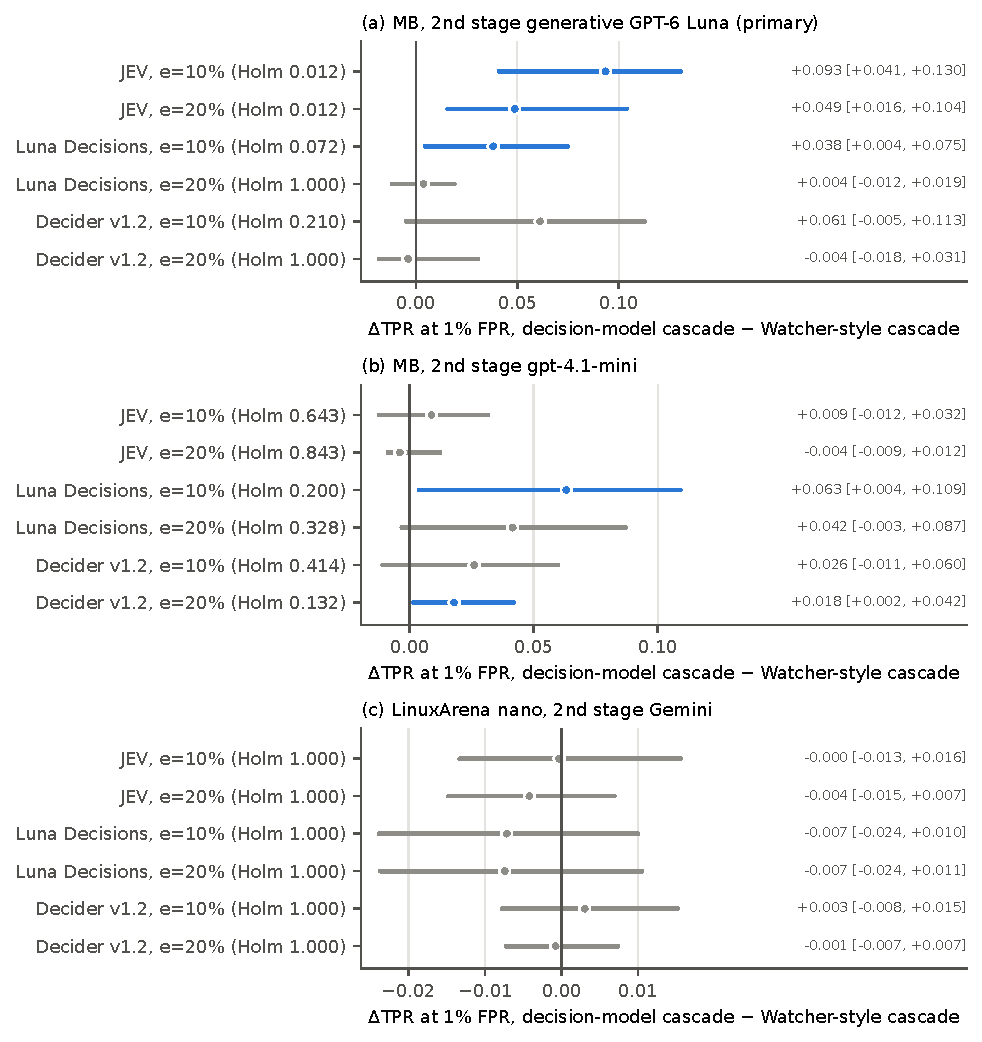
\includegraphics[width=0.8\linewidth]{r5_w12.pdf}
\caption{W1/W2 contrasts (decision-model cascade $-$ Watcher-style cascade, 1\% FPR) on the primary panel (a) and the two secondary panels (b, c). Holm $p$ is within each panel's family of six; only (a) is confirmatory. Conformal rule, main-task resampling (\nolinkurl{results/r5_watch/hypotheses.csv}).}\label{fig:w12}
\end{figure}

\paragraph{W3: Watcher's fixed cutoffs \tE} (pre-specified, descriptive).
\begin{center}\small
\begin{adjustbox}{max width=\linewidth}
\begin{tabular}{@{}llcccccl@{}}
\toprule
Panel & Cutoff & Honest steps & Attack steps & Honest traj. $\ge$1 & Attack traj. & Cascade TPR@1\% (FPR) & Decision models at the same $e$, $\Delta$\\
\midrule
MB, gen & $\ge6$ & 7.4\% & 9.8\% & 76\% & 90\% & 0.349 (1.32\%) & JEV $+0.097$*, Luna $+0.037$, Decider $+0.092$*\\
MB, gen & $\ge8$ & 2.4\% & 5.7\% & 42\% & 74\% & 0.413 (1.42\%) & JEV $+0.033$, Luna $-0.022$, Decider $+0.066$\\
LinuxArena, Gemini & $\ge6$ & 1.3\% & 10.9\% & 37\% & 89\% & 0.818 (0.94\%) & JEV $+0.066$*, Luna $+0.065$*, Decider $+0.101$*\\
LinuxArena, Gemini & $\ge8$ & 0.2\% & 8.3\% & 10\% & 76\% & 0.725 (1.03\%) & JEV $+0.087$*, Luna $+0.054$, Decider $+0.090$*\\
\bottomrule
\end{tabular}
\end{adjustbox}
\end{center}
{\small * 95\% CI excludes 0 (no multiplicity claim; \nolinkurl{results/r5_watch/w3.csv}).}
\begin{itemize}
\item \textbf{Escalation of honest runs.} The cutoff at $\ge6$ escalates at least one step in 76\% of honest MB trajectories, and $\ge8$ does so in 42\%. Under Watcher's defaults, the gateway would see most honest BashArena-style sessions.
\item \textbf{Cost on LinuxArena.} Both cutoffs lose detection relative to Gemini alone: $-0.11$ at $\ge6$ and $-0.20$ at $\ge8$.
\item \textbf{Severity is not suspicion.} The high honest severities are mostly the sudo, firewall and credential work that the MB main tasks require (Figure~\ref{fig:wextra}a). This repeats the round-3 finding of Idea 2 that stakes-only severity is nearly uninformative about sabotage (AUROC 0.53). On LinuxArena honest severity is lower and attack steps are more often $\ge8$.
\end{itemize}

\begin{figure}[H]\centering
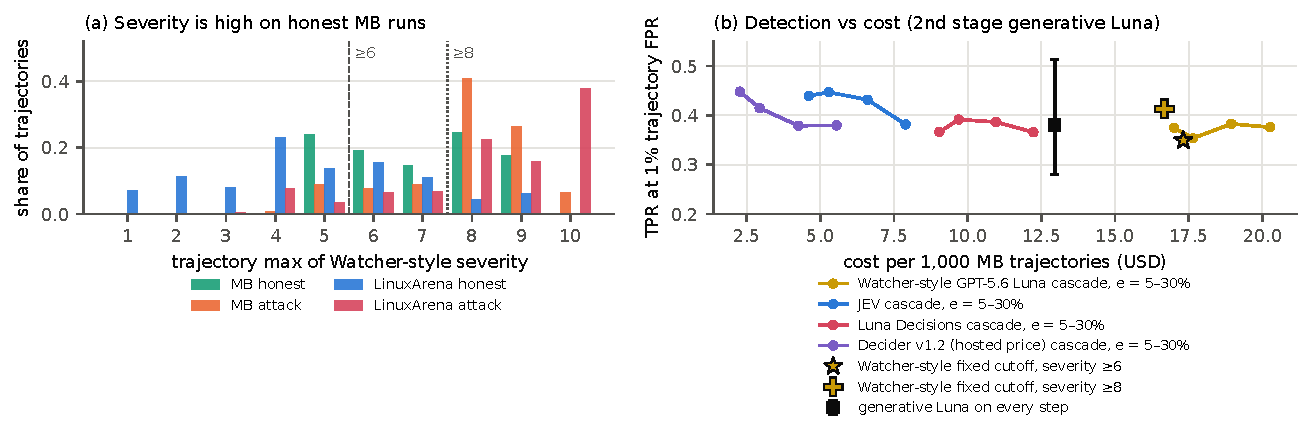
\includegraphics[width=\linewidth]{r5_watch_extra.pdf}
\caption{(a) Distribution of the trajectory maximum of Watcher-style severity, honest vs attack (\nolinkurl{results/r5_watch/explore_severity_hist.csv}). (b) MB, second stage generative GPT-6 Luna: TPR at 1\% FPR vs cost per 1{,}000 trajectories for each first stage's cascade ($e=5$--30\%), Watcher's fixed cutoffs, and generative Luna on every step (\nolinkurl{cells.csv}, \nolinkurl{cost_latency.csv}). Decider is costed at the hosted price; the scores are self-hosted.}\label{fig:wextra}
\end{figure}

\paragraph{Cost and latency} (MB, 29.0 steps per trajectory; generative Luna \$0.00045 per step, median 2.9\,s).
\begin{center}\small
\begin{adjustbox}{max width=\linewidth}
\begin{tabular}{@{}lccccc@{}}
\toprule
First stage & \$/step & Median latency & Alone, \$/1k traj. & Cascade $e=10/20\%$, \$/1k & Serial compute-h/1k, $e=10\%$\\
\midrule
Watcher-style GPT-5.6 Luna & 0.00056 & 0.83\,s & 16.4 & 17.6 / 18.9 (cutoffs: 17.3 / 16.7) & 9.0\\
JEV & 0.00014 & 0.19\,s & 3.9 & 5.3 / 6.6 & 4.0\\
GPT-6 Luna Decisions & 0.00029 & 0.19\,s & 8.4 & 9.7 / 11.0 & 3.9\\
Decider v1.2 (hosted price) & 0.00005 & 0.28\,s & 1.6 & 2.9 / 4.3 & 4.7\\
\midrule
generative GPT-6 Luna on every step & 0.00045 & 2.9\,s & 13.0 & -- & --\\
\texttt{gpt-4.1-mini} on every step & 0.00088 & 2.75\,s & 25.6 & -- & --\\
\bottomrule
\end{tabular}
\end{adjustbox}
\end{center}
\textbf{The Watcher-style triage call costs more per step than the generative GPT-6 Luna second stage.} GPT-5.6 Luna is billed at twice GPT-6 Luna's token prices, and the roughly 2.4k-token rubric is re-sent with every call (only about 46\% of input tokens hit the prompt cache). On these data the Watcher-style cascade therefore costs more than running the second stage on every step. A decision-model cascade costs about half of it, at equal or better detection. Latency numbers are medians from the spend ledger and the caches. They do not include queueing, and the Decider latency is from the hosted dev check.

\section{Shared misses, gate design, the open Decider model and cost}\label{sec:more}

\paragraph{Shared misses \tE.}
\begin{itemize}
\item Attacks that JEV confidently clears (every step $p\le0.05$; 0.6--13.5\% of attacks) are missed by the second-stage LLM far more often than its base rate (Figure~\ref{fig:overlap}): LinuxArena $5.9\times$, iac $3.6\times$, opus-4-6 $1.6\times$, SHADE $1.4\times$, MB $1.1\times$ (mini misses 90\% anyway).
\item Conditional on any JEV miss, the ratios are 1.0--2.7.
\item This matches the rubric-judging result that LLM judges repeat decision models' confident errors, now on sabotage data. Confidence-based escalation therefore cannot rescue confident misses.
\item The intervals hold thresholds at split means and omit threshold noise. Some cells rest on 35--78 attacks.
\end{itemize}
\begin{figure}[H]\centering
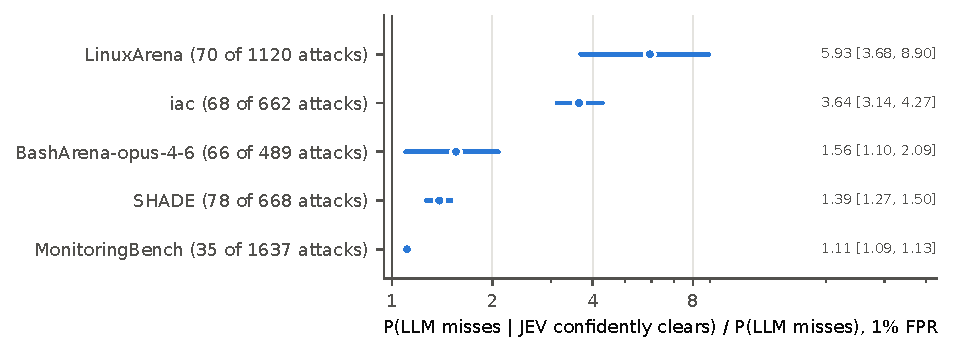
\includegraphics[width=0.72\linewidth]{r5_overlap.pdf}
\caption{Ratio of the second-stage LLM's miss rate on attacks JEV confidently clears to its overall miss rate, 1\% FPR (plug-in thresholds, round-1 exploratory; \nolinkurl{results/r5_jev/explore_rq3_overlap.csv}). Settings where the LLM misses nothing are omitted, as is BashArena-sonnet-4-5 (below the 1\% calibration floor).}\label{fig:overlap}
\end{figure}

\paragraph{Gate design \tE} (round 1, plug-in, 1\% FPR, $e=10\%$).
\begin{itemize}
\item Escalating by suspicion beats escalating the least confident steps everywhere. Confidence gating fails where attack steps get $p\approx1$: bash 0.72 vs 0.99, LinuxArena 0.92 vs 0.94, MB 0.09 vs 0.12.
\item A two-sided rule (escalate the least confident steps, and let $p\ge0.99$ alarm on its own) is about equal to suspicion gating.
\item With full text, the length gate is a cheap complement on settings where payloads sit in long actions (Section~\ref{sec:trunc}).
\end{itemize}

\paragraph{The open Decider model \tE.} Perplexity Decider v1.2 (27B, Apache-2.0) ran on one on-demand H100 at 3.7--4.4 requests/s. It scored MB, the full AK LinuxArena set and the LinuxArena sweep: 219k judgments for about \$67.
\begin{itemize}
\item \textbf{Standalone} it matches JEV. AUROC of the max: MB 0.82 vs 0.81, LinuxArena 0.96 vs 0.94, sweep 0.91 vs 0.88.
\item \textbf{As a router} (round 1, plug-in) it is equal or slightly better. MB 5\%, $e=20\%$: $+0.039\ci{+0.007}{+0.068}$. Sweep at 5\% with \texttt{claude-opus-4-6} as second stage: $+0.05$ (CIs exclude 0 at $e=10$--20\%). With generative Luna on MB it routes like JEV (0.415 vs 0.447 at $e=10\%$, n.s.; W2-decider in Table~\ref{tab:watch}).
\item It returns unrounded probabilities. Self-hosting makes scores reproducible (no silent version changes) and allows white-box reading, which was not done here.
\item The hosted version differs in label-order bias (Section~\ref{sec:luna}).
\end{itemize}

\paragraph{Cost summary.}
\begin{itemize}
\item JEV costs \$0.00004--0.00014 per step across sources (median request about 2.7k tokens, latency about 0.2\,s).
\item Per 1{,}000 MB trajectories: JEV alone \$3.9; nano alone \$6.3; mini alone \$25.6; JEV$\to$mini \$5.3 / 6.7 / 9.3 / 11.8 at $e=5/10/20/30\%$; JEV$\to$generative Luna \$5.3 / 6.6 at $e=10/20\%$ vs \$13.0 for Luna alone.
\item On AK LinuxArena, $e=20\%$ cuts LLM calls from 57.8k to 11.6k per 1{,}000 trajectories.
\item Luna Decisions costs \$0.00011--0.00030 per step, two to three times JEV's cost on the same requests.
\end{itemize}

\section{Claims ledger}\label{sec:ledger}
\tC\ = preregistered test; \tE\ = exploratory, secondary or descriptive. Conformal rule unless noted.
{\footnotesize
\begin{xltabular}{\linewidth}{@{}>{\raggedright\arraybackslash}p{4.6cm}c>{\raggedright\arraybackslash}p{3.6cm}>{\raggedright\arraybackslash}X@{}}
\toprule
Claim & Tag & Estimate [95\% CI] & Caveat\\
\midrule
\endhead
JEV triage beats nano triage on AK (H2-AK) & \tC & $+0.170\ci{+0.131}{+0.201}$ & Compares designs (window + rubric vs history-free prompt)\\
JEV triage $\approx$ nano triage on MB (H2-MB) & \tC & $-0.000\ci{-0.042}{+0.032}$; not supported & Weak second stage\\
JEV cascade non-inferior to Gemini alone, AK pooled (H1-AK) & \tC & $+0.005\ci{-0.014}{+0.028}$ & Cancellation (SHADE $+0.18$, opus-4-6 $-0.22$); not NI without SHADE ($-0.023$) or at 5\% ($-0.025$)\\
JEV cascade non-inferior to mini alone on MB (H1-MB) & \tC & $-0.002\ci{-0.006}{+0.002}$ & Degenerate panel (mini TPR 0.10)\\
JEV triage non-inferior to probe triage on MB (H3-MB) & \tC & $+0.008\ci{-0.005}{+0.032}$ & Degenerate panel\\
JEV$\to$generative Luna non-inferior to Luna alone on MB (H1-MB-strong) & \tC & $+0.051\ci{-0.004}{+0.106}$ & Superiority not shown; one benchmark\\
Luna Decisions routes worse than JEV on AK (H5a-AK) & \tC & $-0.034\ci{-0.056}{-0.021}$ & Driven by iac, agentdojo; MB n.s.\\
Luna Decisions routes worse than JEV into Luna on MB (T2, $e=20\%$) & \tC & $-0.045\ci{-0.098}{-0.014}$ & $e=10\%$ n.s.\\
Luna Decisions triage beats nano triage on AK (H5b-AK) & \tC & $+0.130\ci{+0.090}{+0.165}$ & Compares designs\\
Interface penalty: Luna Decisions below generative Luna (H5c) & \tC & $-0.158\ci{-0.227}{-0.113}$; MB $-0.343$ & Prompt wording, caps and reasoning also differ\\
Full text raises opus-4-6 AUROC and cascade TPR (H5d) & \tC & AUROC $+0.107$; cascade $+0.110\ci{+0.059}{+0.150}$ & Standalone AUROC stays $<0.5$\\
Full-text JEV cascade matches Gemini on opus-4-6 & \tE & 0.492$\to$0.755 vs Gemini 0.710 & Secondary cell; no direct CI vs Gemini\\
Generative Luna beats Luna Decisions and Decider standalone on MB (S2, S3) & \tC & $+0.338$, $+0.218$ & S1 (vs JEV) and S4 (vs probe) n.s.\\
JEV beats Watcher-style triage into Luna on MB (W1) & \tC & $+0.093\ci{+0.041}{+0.130}$; $+0.049\ci{+0.016}{+0.104}$ & Published rubric, not Watcher Live; MB only\\
Luna Decisions, Decider vs Watcher-style (W2) & \tC & $+0.038$, $+0.061$ at 10\%; $\approx0$ at 20\% & Not significant after Holm\\
Watcher-style cutoffs escalate most honest MB runs (W3) & \tE & $\ge6$: 76\%; $\ge8$: 42\% of honest trajectories & Severity tracks stakes, not intent\\
Watcher-style triage costs more than Luna on every step & \tE & \$17.6--18.9 vs \$13.0 per 1k traj. & Prices as of Oct 2026; effort \texttt{none}\\
Standalone JEV beats mini on MB & \tE & not shown at equal FPR ($+0.074\ci{-0.013}{+0.205}$) & JEV floor 2.2\% realized FPR\\
MB 5\%: small-$e$ JEV/probe cascades beat mini & \tE & $+0.017$, $+0.021$, $+0.007$ at equal FPR; n.s. & Nominal gains were at unequal FPR\\
Length explains the opus-4-6 inversion & \tE & no: 0.30$\to$0.35--0.36 within strata & Post hoc firewall/truncation checks\\
Confident JEV misses are shared with the LLM & \tE & ratio 1.1--5.9 & Threshold noise omitted\\
Suspicion gating $\ge$ confidence gating & \tE & e.g.\ bash 0.99 vs 0.72 & Plug-in, one $e$\\
Decider routes as well as JEV & \tE & AUROC 0.82 vs 0.81 (MB); router $\ge$ JEV & Plug-in; hosted version differs\\
No monitor sees agent reasoning & -- & audit 3 & Step count is label-correlated\\
\bottomrule
\end{xltabular}}

\section{Limitations}\label{sec:lim}
\begin{itemize}
\item \textbf{Offline replay of public benchmarks.} Every result is computed on fixed, already-generated trajectories (MonitoringBench, aksh-n, the LinuxArena sweep). Nothing was deployed, and no attack was executed for this idea.
\item \textbf{No adaptive attacker.} Attacks that target the decision model were not run. Whether a trajectory-level attacker who knows a decision model is the first stage can pass it is an open question. The single-input steering results in the literature and the truncation finding here both suggest it matters.
\item \textbf{Possible benchmark contamination.} JEV, Luna, Decider and the LLM monitors may have seen these public benchmarks in training. This cannot be checked.
\item \textbf{Beta and closed model versions.} JEV 1.14 and GPT-6 Luna Decisions are pinned by versioned id but are closed and recent (Luna Decisions is a public beta). Results may not transfer to later versions. The hosted Decider already differs from the self-hosted one.
\item \textbf{External second-stage scores were not reproduced.} The AK Gemini scores and the LinuxArena sweep monitors are the dataset authors' outputs. We cannot verify their inputs; for example, if the AK LinuxArena judge saw agent reasoning, its baseline is inflated. Those scores were computed on full text, unlike our first stages.
\item \textbf{Heterogeneity across settings.} Pooled AK results average over settings that behave very differently (SHADE vs opus-4-6, iac for Luna), and several settings have few main tasks (SHADE 5, iac 5, agentdojo 16). Main-task resampling widens intervals there.
\item \textbf{Weak and shared baselines.} The MB comparisons in round 1 use a weak second stage. Honest-550 is entirely \texttt{claude-opus-4-5}, and all panels reuse data from earlier tracks.
\item \textbf{The Watcher arm is a reconstruction}, run at effort \texttt{none} chosen for cost on 20 dev trajectories, and its dev AUROC overstated held-out.
\item \textbf{Design differences in H2, H5b and H5c} are declared but not separated from the model or interface effects.
\end{itemize}

\section{Next steps}\label{sec:next}
\begin{enumerate}
\item \textbf{Full-text or chunked first stages.} Re-run H1-AK with full-text JEV on all AK settings, plus a cheap length gate as a complement, and test whether the cancellation disappears.
\item \textbf{Separate interface from prompt in H5c.} Run generative Luna with the decision request's exact text and caps, and with reasoning disabled.
\item \textbf{Strong second stages on more panels.} Generative Luna or another frontier monitor on AK and LinuxArena, where the dataset's Gemini scores are external and full-text.
\item \textbf{A faithful Watcher comparison.} Use Watcher's own context assembly (whole conversation, no tool outputs) and reasoning effort, or Watcher Live itself if access allows, on sessions closer to its design target.
\item \textbf{Open-model follow-ups.} Order-averaged Decider scores; white-box reading or fine-tuning of the open model on monitoring labels with whole settings held out.
\item \textbf{Robustness.} Test whether a trajectory-level attacker who knows the first stage can pass it, with an uninformed-rewrite control and execution validity (the Idea 3 machinery).
\end{enumerate}

\section*{Cost and reproduction}
\begin{itemize}
\item \textbf{OpenRouter} (repository spend ledger): r5dev \$5.34 (JEV dev variants); r5jev \$82.08 (JEV held-out \$47.04, \texttt{gpt-4.1-nano} \$35.04); r5luna \$154.38 (Luna Decisions frozen \$92.92, generative Luna \$56.63, full-text arms \$3.75, dev and checks \$1.08); r5watch \$61.90 (MB \$36.10, LinuxArena \$23.10, dev \$2.70). Total \textbf{\$303.70}.
\item \textbf{RunPod} (MATS account, on-demand): one H100 for Decider, about 16.9\,h at \$3.99/h $\approx$ \$67. The pod was deleted after outputs were copied off and verified.
\item \textbf{Code:} \texttt{tracks/r5\_jev/}, \texttt{tracks/r5\_luna/}, \texttt{tracks/r5\_watch/}, \texttt{tracks/audit3/} (\texttt{jev\_*}), \texttt{tracks/fixes2/} (\texttt{jev\_*}); report figures \texttt{docs/reports/src/make\_r5\_report\_figs.py}.
\item \textbf{Results:} \texttt{results/r5\_jev/}, \texttt{results/r5\_luna/}, \texttt{results/r5\_watch/}, \texttt{results/audit3/}, \texttt{results/fixes2/}.
\item \textbf{Log:} \texttt{EXPERIMENT\_LOG.md} (22--24 Oct 2026). Repository: \url{https://github.com/gregkocher/agent-monitor-detection} (private).
\end{itemize}
\end{document}
